\documentclass[12pt]{article}

\usepackage[brazilian]{babel}
\usepackage[utf8]{inputenc}
\usepackage{graphicx}
\usepackage{mathtools}
\usepackage{amsthm}
\usepackage{amssymb}
\usepackage{thmtools,thm-restate}
\usepackage{amsfonts}
\usepackage{hyperref}
\usepackage[singlelinecheck=false]{caption}
\usepackage[backend=biber,url=true,doi=true,eprint=false,style=numeric]{biblatex}
\usepackage{enumitem}
\usepackage[justification=centering]{caption}
\usepackage{indentfirst}
\usepackage{algorithm}
\usepackage[noend]{algpseudocode}
\usepackage{listings}
\usepackage[x11names,rgb,table]{xcolor}
\usepackage{tikz}
\usepackage{hyperref}
\usepackage{subcaption}
\usepackage{booktabs}
\usepackage{linegoal}
\usepackage{geometry}
\usetikzlibrary{snakes,arrows,shapes}

\addbibresource{references.bib}
\graphicspath{{imgs/}}

\makeatletter
\def\subsection{\@startsection{subsection}{3}%
  \z@{.5\linespacing\@plus.7\linespacing}{.1\linespacing}%
  {\normalfont}}
\makeatother

\makeatletter
\patchcmd{\@setauthors}{\MakeUppercase}{}{}{}
\makeatother

\DeclareMathOperator*{\argmin}{arg\,min}
\DeclareMathOperator*{\argmax}{arg\,max}
\DeclareMathOperator*{\Val}{\text{Val}}
\DeclareMathOperator*{\Ch}{\text{Ch}}
\DeclareMathOperator*{\Pa}{\text{Pa}}
\DeclareMathOperator*{\Sc}{\text{Sc}}
\newcommand{\ov}{\overline}
\newcommand{\tsup}{\textsuperscript}

\newcommand\defeq{\mathrel{\overset{\makebox[0pt]{\mbox{\normalfont\tiny\sffamily def}}}{=}}}

\newcommand{\algorithmautorefname}{Algorithm}
\algrenewcommand\algorithmicrequire{\textbf{Entrada}}
\algrenewcommand\algorithmicensure{\textbf{Saída}}
\algrenewcommand\algorithmicif{\textbf{se}}
\algrenewcommand\algorithmicthen{\textbf{então}}
\algrenewcommand\algorithmicelse{\textbf{senão}}
\algrenewcommand\algorithmicfor{\textbf{para todo}}
\algrenewcommand\algorithmicdo{\textbf{faça}}
\algnewcommand{\LineComment}[1]{\State\,\(\triangleright\) #1}

\captionsetup[table]{labelsep=space}

\theoremstyle{plain}

\newcounter{dummy-def}\numberwithin{dummy-def}{section}
\newtheorem{definition}[dummy-def]{Definition}
\newcounter{dummy-thm}\numberwithin{dummy-thm}{section}
\newtheorem{theorem}[dummy-thm]{Theorem}
\newcounter{dummy-prop}\numberwithin{dummy-prop}{section}
\newtheorem{proposition}[dummy-prop]{Proposition}
\newcounter{dummy-corollary}\numberwithin{dummy-corollary}{section}
\newtheorem{corollary}[dummy-corollary]{Corollary}
\newcounter{dummy-lemma}\numberwithin{dummy-lemma}{section}
\newtheorem{lemma}[dummy-lemma]{Lemma}
\newcounter{dummy-ex}\numberwithin{dummy-ex}{section}
\newtheorem{exercise}[dummy-ex]{Exercise}
\newcounter{dummy-eg}\numberwithin{dummy-eg}{section}
\newtheorem{example}[dummy-eg]{Example}

\numberwithin{equation}{section}

\newcommand{\set}[1]{\mathbf{#1}}
\newcommand{\pr}{\text{P}}
\newcommand{\eps}{\varepsilon}
\newcommand{\ddspn}[2]{\frac{\partial#1}{\partial#2}}
\newcommand{\iddspn}[2]{\partial#1/\partial#2}
\newcommand{\indep}{\perp}
\renewcommand{\implies}{\Rightarrow}

\newcommand{\bigo}{\mathcal{O}}

\setlength{\parskip}{1em}

\lstset{frameround=fttt,
	numbers=left,
	breaklines=true,
	keywordstyle=\bfseries,
	basicstyle=\ttfamily,
}

\newcommand{\code}[1]{\lstinline[mathescape=true]{#1}}
\newcommand{\mcode}[1]{\lstinline[mathescape]!#1!}

\newgeometry{margin=1in}
\title{%
  \vspace{-3.0cm}
  {
\includegraphics[scale=0.2]{logo-usp.png}}\\
  {\textbf{\uppercase{\Large USP --- Universidade de São Paulo}}}\\
  \vspace{1.5cm}
  {\textbf{Aprendizagem automática de redes soma-produto}}\\
  \vspace{2.0cm}
\flushleft{\Large Relatório Final de Projeto de Iniciação Científica\\
CNPq PIBIC Projeto 800585/2016\texttt{-}0}\\
  \vspace{2.5cm}
\flushleft{\Large Bolsista: Renato Lui Geh\\
Orientador: Prof.\ Dr.\ Denis Deratani Mauá}\\
  \vspace{2.5cm}
  \centering
  {\Large\textbf{São Paulo}}\\
  \vspace{0.25cm}
  {\Large\textbf{2018}}\\
}
\date{}

\begin{document}

\maketitle

\renewcommand{\abstractname}{\Large{Resumo}}

\begin{abstract}
  \vspace{0.4cm}
  \normalsize
  Modelos probabilísticos baseados em grafo (PGMs) possibilitam modelar distribuições de
  probabilidade complexas com milhares de varíaveis. Devido a grande expressividade em
  representabilidade, PGMs mostraram-se viáveis para modelagem de casos reais.

  Redes soma-produto (SPNs) são PGMs que restringem-se ao escopo de distribuições de probabilidade
  tratáveis. SPNs tiveram bons resultados em diversas aplicações, obtendo valores comparáveis a
  outros modelos estado-da-arte, porém com tempo de execução ordens de magnitude menor.

  Apesar dos resultados promissores, atualmente existem poucas bibliotecas para inferência e
  aprendizado de SPNs. Além disso, não existe atualmente uma comparação detalhada entre diferentes
  algoritmos de rede-soma produto.

  Este projeto teve dois objetivos. O primeiro foi construir uma biblioteca livre e gratuita para
  inferência e aprendizado de redes soma-produto. O segundo foi fazer uma comparação de alguns
  algoritmos de aprendizado de SPNs no domínio de classificação e compleição de imagens.\\~\\

  \textbf{Palavras-chave:} Modelos probabilísticos baseados em grafo, redes soma-produto,
  processamento de imagens
  \newpage
\end{abstract}

\section{Introdução}

Modelos probabilísticos baseados em grafos (PGM, do inglês \textit{Probabilistic Graphical Models})
representam uma distribuição de probabilidade de forma compacta. Estes modelos representados por
grafos facilitam tanto a compreensão humana ao estudá-los, quanto possibilitam que vários problemas
já existentes em Teoria dos Grafos sejam utilizados como solução para problemas em PGMs. Extrair
conhecimento de PGMs é análogo a extrair a probabilidade de um certo evento ocorrer dado que
eventos distintos tenham ocorrido. Tal extração de conhecimento é chamada de inferência. Fazer
inferência exata em PGMs clássicas, ou seja, achar a probabilidade exata de um certo evento, é
intratável. Uma solução para este problema é utilizar métodos para inferência aproximada nestes
modelos. No entanto, tais algoritmos aproximados são muitas vezes difíceis de analisar. Além disso,
como os algoritmos de aprendizado do modelo utilizam inferência como subrotina, por consequência o
aprendizado torna-se aproximado.

\begin{figure}[h]
  \centering
  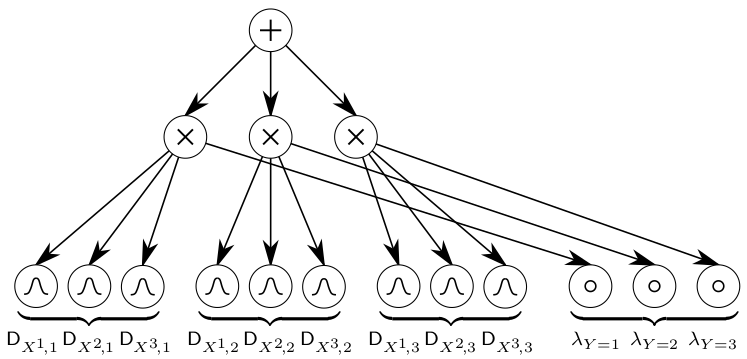
\includegraphics[scale=0.4]{nbayes.png}
  \caption{Fonte~\cite{peharz-spn}}\label{spn-example}
\end{figure}

Redes soma-produto (SPN, de \textit{Sum-Product Network}) são PGMs que representam uma distribuição
de probabilidade tratável. Proposto em 2011, SPNs computam inferência exata em tempo linear ao
número de arestas de seu grafo se sua estrutura obedecer a certas
propriedades~\cite{poon-domingos}. A~\autoref{spn-example} mostra um exemplo de rede soma-produto
representando o modelo Naïve Bayes com três atributos. SPNs apresentam uma série de características
interessantes, como sua arquitetura profunda que permite representar funções de forma mais
eficiente quanto mais profundo seu grafo~\cite{shallow-vs-deep}. Outras interessantes propriedades
teóricas incluem uma generalização de SPNs para qualquer semianel em que o produto tenha escopo
disjunto~\cite{sp-theorem}. Com relação a aplicações, SPNs tiveram resultados impressionantes em
diversas áreas, como enovelamento de proteínas~\cite{rec-dec-non-convex}, modelagem de
sinais~\cite{model-speech}, classificação e reconstrução de
imagens~\cite{gens-domingos,poon-domingos,clustering}, reconhecimento de atividade~\cite{activity}
e linguagem natural~\cite{nat-lang}.

Uma SPN pode ser definida como um DAG onde nós são somas ponderadas, produtos, variáveis
indicadoras ou distribuições de probabilidade univariadas. Uma folha de uma SPN é
sempre uma variável indicadora ou uma distribuição univariada e vice-versa. O escopo de uma SPN é o
conjunto de todas variáveis da rede. O escopo de uma folha de uma SPN é a variável descrita pela
variável indicadora ou distribuição univariada. Semânticamente, o conjunto de filhos de um nó soma
pode ser interpretado como uma relação de semelhança entre as variáveis dos escopos dos filhos,
enquanto que o conjunto de filhos de um produto pode ser visto como uma relação de independência
entre os escopos dos filhos do nó produto. O valor de um nó soma é a soma ponderada de seus filhos
em função dos pesos de suas arestas de saída. O valor de um nó produto é o produto dos valores dos
filhos e o valor de uma folha é o valor da variável indicadora ou a probabilidade da distribuição
univariada.

Apesar dos resultados expressivos, atualmente existem poucas bibliotecas para inferência e
aprendizado de redes soma-produto. Grande parte dos códigos existentes possuem pouca documentação
ou não são mais mantidos ou atualizados. Além disso, não existem comparações detalhadas entre
algoritmos de aprendizado de SPNs na literatura ou uma biblioteca que facilite esta tarefa.

Neste projeto, buscou-se criar uma biblioteca livre e gratuita para inferência e aprendizado de
redes soma-produto. Foram implementadas subrotinas para computar a probabilidade de evidência
exata, a probabilidade \textit{maximum a posteriori} aproximada de uma SPN e três métodos de
aprendizado de redes soma-produto. Adicionalmente, foram implementadas funções para auxiliar a
comparação entre diferentes arquiteturas de SPNs, verificar propriedades da estrutura da rede e
classificar e completar imagens.

\section{Objetivos}

O projeto teve como objetivos criar uma biblioteca livre e gratuita para inferência e aprendizado
de redes soma-produto e gerar dados comparativos de diversos algoritmos de aprendizado de SPNs
estado-da-arte.

Originalmente, planejava-se implementar quatro algoritmos de aprendizado. No entanto, preferiu-se
gerar um relatório mais detalhado de três algoritmos. Os três algoritmos implementados são listados
abaixo.

\begin{enumerate}[label=\alph*.]
  \item Algoritmo de Poon-Domingos~\cite{poon-domingos}
  \item Algoritmo de aprendizado estrutural de Dennis-Ventura~\cite{clustering}
  \item Algoritmo de aprendizado estrutural de Gens-Domingos~\cite{gens-domingos}
\end{enumerate}

Após as implementações, foram feitos testes de desempenho em conjuntos de dados reais e artificiais
para classificação e compleição de imagens.

\section{Metodologia}

Neste projeto, buscou-se analisar três artigos de aprendizado de redes soma-produto.

\begin{enumerate}
  \item \textit{Sum-Product Networks: A New Deep Architecture}, H. Poon e P. Domingos, UAI
    2011~\cite{poon-domingos}
  \item \textit{Learning the Structure of Sum-Product Networks}, R. Gens e P. Domingos, ICML
    2013~\cite{gens-domingos}
  \item \textit{Learning the Architecture of Sum-Product Networks Using Clustering on Variables},
    A. Dennis e D. Ventura, NIPS 2012~\cite{clustering}
\end{enumerate}

Foram implementados os algoritmos descritos e tentou-se replicar os resultados apresentados nos
artigos. Para isso, foi construída a biblioteca
GoSPN\footnote{\url{https://github.com/RenatoGeh/gospn}} na linguagem Go. A escolha da linguagem
foi dada pelo suporte nativo a programação concorrente e paralela, velocidade de execução, e por
ser uma linguagem fortemente tipada e compilada.

Após implementados os métodos de aprendizagem, foram feitos testes e comparações nos desempenhos e
acurácias dos três algoritmos nos seguintes conjuntos de dados de imagens.

\begin{enumerate}[label=\,(\alph*)]
  \item Caltech-101~\cite{caltech101}
  \item Olivetti Faces Dataset~\cite{olivetti}
  \item Digits~\cite{digits}
  \item DigitsX~\cite{digitsx}
  \item MNIST~\cite{mnist}
\end{enumerate}

\section{Resultados e discussão}

O projeto consistiu na elaboração de três algoritmos de aprendizado. Estes algoritmos foram
implementados na biblioteca GoSPN\footnotemark[1]. Duas variações do método de otimização de
descida de gradiente foram escritas para os algoritmos de Poon-Domingos e Dennis-Ventura. Para o
algoritmo de Gens-Domingos, foram implementados dois métodos de \textit{clustering}, DBSCAN e
$k$-means. Adicionalmente, os algoritmos $k$-mode e $k$-medoid foram implementados por Diarmaid
Conaty\footnotemark[2] e Cassio P. de Campos\footnote{Queen's University Belfast} como
contribuições à biblioteca. Para os testes de independência entre variáveis foram implementados os
testes de qui-quadrado e G-test. A biblioteca também possibilita o uso de distribuições gaussianas
ou multinomiais como folhas da rede.

Para o método de otimização de descida de gradiente, foram criadas as versões \textit{soft} e
\textit{hard}. A primeira usa as derivadas parciais da SPN em função dos pesos para atualizar os
parâmetros da rede. No entanto, para o caso de redes profundas o gradiente tende a se aproximar de
zero conforme o sinal é propagado pela rede. Para evitar este problema, usa-se o segundo método.
Seja $S$ uma SPN, define-se $M$ a rede máximo-produto (MPN) de $S$ como o grafo cópia de $S$ em que
todos os nós somas são substituidos por nós máximo. O valor de um nó máximo é o maior valor
ponderado de seus filhos. O valor de uma MPN é o valor da raíz. O caminho percorrido a partir da
raíz de maior valor representa a probabilidade \textit{maximum a posteriori} (MAP). Denotaremos
por $W$ o multiconjunto de todas as arestas que pertencem ao caminho descrito pelo MAP\@. Extraindo
as derivadas da MPN $M$ e denotando $\Ch(n)$ e $\Pa(n)$ os conjuntos de filhos e pais do nó $n$
respectivamente, temos os valores descritos nas tabelas~\ref{tab:derivative-spn}
e~\ref{tab:derivative-weight}.

\begin{table}[h]
  \centering
  \begin{tabular}{l|l}
    \hline
    \multicolumn{1}{c}{\bfseries Método} & \multicolumn{1}{c}{\bfseries Derivada parcial do nó $j$}\\
    \hline & \\
    \textbf{Soft} & \(\displaystyle \ddspn{S}{S_j}=\sum_{\substack{n\in\Pa(j)\\n:\text{ soma}}}w_{n,j}\ddspn{S}{S_n}+\sum_{\substack{n\in\Pa(j)\\n:\text{ produto}}}\ddspn{S}{S_n}\prod_{k\in\Ch(n)\setminus\{j\}}S_k\) \\
    & \\
    \textbf{Hard} & \(\displaystyle
        \ddspn{M}{M_j}=\sum_{\substack{n\in\Pa(j)\\n:\text{ soma}}}
        \begin{cases}
          w_{k,n}\ddspn{M}{M_k} & \text{se $w_{k,n}\in W$}\\
          0 & \text{c.c.}
        \end{cases}
        + \sum_{\substack{n\in\Pa(j)\\n:\text{ produto}}}\ddspn{M}{M_n}\prod_{k\in\Ch(n)\setminus\{j\}}M_k
      \) \\
      & \\
    \hline
  \end{tabular}
  \caption{\label{tab:derivative-spn} As derivadas parciais da SPN em função de um nó $j$ no caso
    geral.}
\end{table}

\begin{table}[h]
  \centering
  \begin{tabular}{l|c}
    \hline
    \multicolumn{1}{c}{\bfseries Método} & \multicolumn{1}{c}{\bfseries Derivada parcial do peso}\\
    \hline & \\
    \textbf{Soft} & \(\displaystyle \ddspn{S}{w_{n,j}} = S_j\ddspn{S}{S_n} \) \\
    & \\
    \textbf{Hard} & \(\displaystyle \ddspn{M}{w_{n,j}} = M_j\ddspn{M}{M_n} \) \\
    & \\
    \hline
  \end{tabular}
  \caption{\label{tab:derivative-weight} As derivadas parciais da SPN em função da aresta $n\to j$.}
\end{table}

Todas as derivadas são em função de certa evidência. Portanto a notação $\iddspn{S}{S_j}$ equivale a
$\iddspn{S}{S_j}(X)$, onde $X$ é algum conjunto de valorações válidas para as variáveis de $S$.
Para computar o gradiente, deriva-se a log-verossimilhança da distribuição da SPN em função do
conjunto de parâmetros $w$, ou seja, $\ddspn{}{w}\log\pr(X)$, obtendo os resultados
da~\autoref{tab:gradients}.

\begin{table}[H]
  \centering
  \begin{tabular}{l|c}
    \hline
    \multicolumn{1}{c}{\bfseries Método} & \multicolumn{1}{c}{\bfseries Gradientes}\\
    \hline & \\
    \textbf{Soft} & \(\displaystyle \Delta w_{n,j} = \eta\ddspn{S}{w_{n,j}} \) \\
    & \\
    \textbf{Hard} & \(\displaystyle \Delta w_{n,j} = \eta \frac{c_{n,j}}{w_{n,j}} \) \\
    & \\
    \hline
  \end{tabular}
  \caption{\label{tab:gradients} As atualizações dos pesos da SPN a partir do gradiente para cada
    aresta $n\to j$.}
\end{table}

Onde $c_{n,j}$ denota a contagem de vezes que $w_{n,j}$ pertence a $W$. No caso do método
\textit{soft} de gradiente descendente, a atualização do peso depende da derivada parcial
$\iddspn{S}{w_{n,j}}$, enquanto que na versão \textit{hard}, $\Delta w_{n,j}$ apenas depende do
número de passagens pela aresta. É portanto possível perceber o porquê do método \textit{soft}
ter problemas com difusão de gradiente e \textit{hard} não. Testes feitos com todos os conjuntos de
dados usados mostraram que difusão de gradiente ocorreu em todos eles, o que mostra que, em
casos de mundo real é necessário o uso do método de otimização de gradiente descendente
\textit{hard}.

\begin{figure}[h]
  \begin{subfigure}{.5\textwidth}
    \centering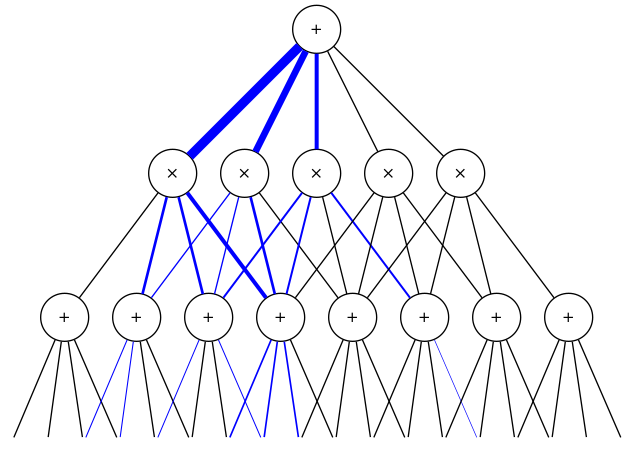
\includegraphics[scale=0.375]{graphs/softgrad.png}
    \caption{Derivação \textit{soft}}
  \end{subfigure}
  \begin{subfigure}{.5\textwidth}
    \centering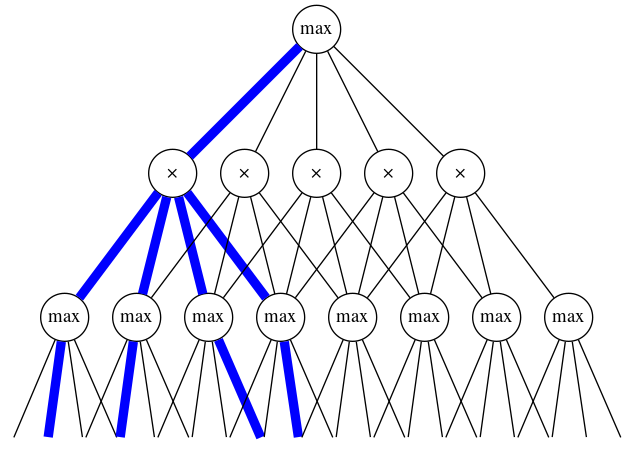
\includegraphics[scale=0.375]{graphs/hardgrad.png}
    \caption{Derivação \textit{hard}}
  \end{subfigure}
  \captionsetup{justification=raggedright}
  \caption{O gradiente no método \textit{soft} tende a se diluir conforme a altura da rede. Usando
  a derivação \textit{hard}, o gradiente não depende da derivada parcial diluída.}
\end{figure}

Para a implementação e replicação dos resultados do artigo de Poon-Domingos, foi necessário
implementar o algoritmo de geração de estrutura densa descrito no artigo. O código escrito para
este algoritmo é restrito ao domínio de imagens, no entanto, a ideia por trás da arquitetura pode
ser aplicada a qualquer domínio em que existe uma forte relação de dependência entre variáveis
locais~\cite{poon-domingos}.

A estrutura densa é formulada a partir da ideia de que existe uma relação de semelhança entre
os pixels de uma região retangular de uma imagem, e uma relação de independência entre outras
regiões retangulares que não a contém. Cada região retangular é representada por um conjunto de $m$
nós somas. Para cada região retangular, decompõe-se a região em duas partições de forma que as
partições também sejam regiões retangulares da imagem. Na SPN, representa-se esta decomposição por
um conjunto de nós produtos.

\begin{figure}[h]
  \centering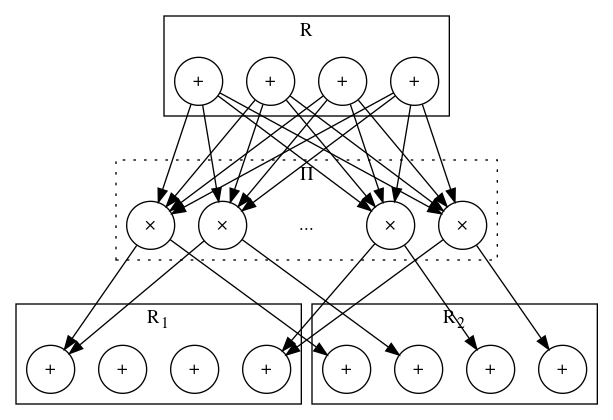
\includegraphics[scale=0.5]{graphs/decomp.png}
  \captionsetup{justification=raggedright}
  \caption{Decomposição de uma região $R$ em duas subregiões $R_1$ e $R_2$. O conjunto $\Pi$ de nós
  produtos representa a relação de independência entre as duas subregiões.}
\end{figure}

Quando $R$ representa a própria imagem, ou seja, a região retangular que engloba todos os pixels da
imagem, então o conjunto de nós somas contém apenas um nó soma. Para regiões unitárias em que a
região é apenas um pixel, ao invés de somas, geram-se $g$ gaussianas de tal forma que cada $k$
gaussiana é o $k$-ésimo quantil da distribuição dos valores do pixel. Quando a região tem dimensões
menores que $r\times r$, a chamamos de região fina. As regiões maiores ou iguais a $r\times
r$ são chamadas de regiões grosseiras. Para as regiões grosseiras tomam-se apenas partições que
geram subregiões maiores ou iguais a $r\times r$, enquanto que para regiões finas, geram-se
partições para todas as possíveis subregiões retangulares. As arestas conectando uma região $R$ ao
conjunto de produtos $\Pi$ são geradas de tal forma que todo nó soma de $R$ está conectada a todo
nó produto de $\Pi$. Porém, as arestas ligando cada produto em $\Pi$ a cada nó soma nas subregiões
$r_1$ e $R_2$ podem ou não existir. Para decidir quais arestas devem existir, escolhe-se uma
ligação $\pi_k\to\sigma_j^i$, onde $\pi\in\Pi$ e $\sigma_j^i\in R_j$, tal que esta aresta seja a
mais provável dada uma instância do conjunto de treinamento.

No código disponibilizado pelos autores do
artigo\footnote{http://spn.cs.washington.edu/spn/downloadspn.php}, o algoritmo usa \textit{hard}
Expectation-Maximization (EM) para gerar as arestas mais prováveis e decidir seus pesos, apesar do
artigo dar resultados para o método de otimização de gradiente descendente. Com o intuito de gerar
resultados mais semelhantes ao artigo possível, foi implementada a parte de se gerar as arestas
mais prováveis por \textit{hard} EM, porém a ponderação das arestas foi feita a partir do método de
gradiente.

O algoritmo de Dennis-Ventura segue uma ideia similar ao de Poon-Domingos, buscando achar relações
de semelhança e independência entre regiões da imagem. No entanto, generaliza-se a ideia de região
para qualquer conjunto de pixels similares, mesmo que não sejam localmente próximas, e podendo
tomar formas arbitrárias. Para isso, usa-se métodos de clustering para achar tais regiões.

Seja $D$ o conjunto de dados, onde $D_i$ é a $i$-ésima instância. $D_i$ então descreve um conjunto
ordenado de valorações dos pixels (ou seja, uma imagem) indexado pelos pixels. É possível
visualizar $D$ como uma matriz $n\times m$, onde $n$ é o número de imagens do conjunto de dados e
$m$ é o número de pixels na imagem. A transposta de $D^\intercal$ é portanto a matriz $m\times n$,
onde as colunas são as imagens e as linhas as valorações de um mesmo pixel.

Para o algoritmo de Dennis-Ventura, gera-se inicialmente um ``grafo de regiões'' que descreve a SPN
por meio de um esboço da arquitetura final. Um nó no grafo de regiões é um nó região ou um nó
partição. A raíz do grafo é sempre a imagem inteira. O grafo de regiões é gerado particionando-se,
recursivamente, cada região em duas subregiões. Seja $R$ um nó região e $D_R^\intercal$ o conjunto
de dados transposto contendo apenas variáveis no escopo de $R$, particiona-se $R$ em duas
subregiões $R_1$ e $R_2$ usando $2$-means clustering em $D_R^\intercal$. O resultado deste
clustering são os dois conjuntos de dados transpostos $D_{R_1}^\intercal$ e $D_{R_2}^\intercal$.
Cria-se um nó partição $P$ e liga-se $R\to P$, $P\to R_1$ e $P\to R_2$. Em seguida, faz-se a
recorrência em $R_1$ e $R_2$ se, para cada região, seu escopo for maior que um. Para o nó raíz,
repetem-se estes passos $k$ vezes, onde a cada passo $i$, usa-se o $i$-ésimo cluster de um
$k$-cluster em $D$ (não transposto).

\begin{figure}[h]
  \begin{subfigure}{.4\linewidth}
    \centering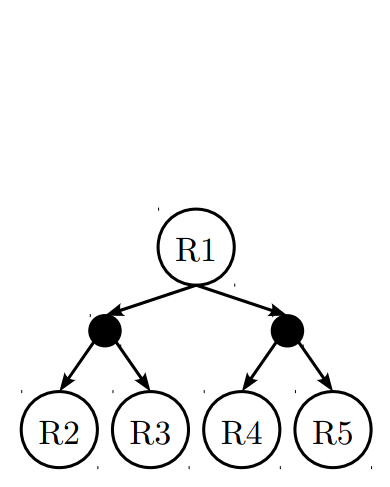
\includegraphics[scale=1.0]{imgs/simple_dv.png}
    \caption{}
  \end{subfigure}
  \begin{subfigure}{.6\linewidth}
    \centering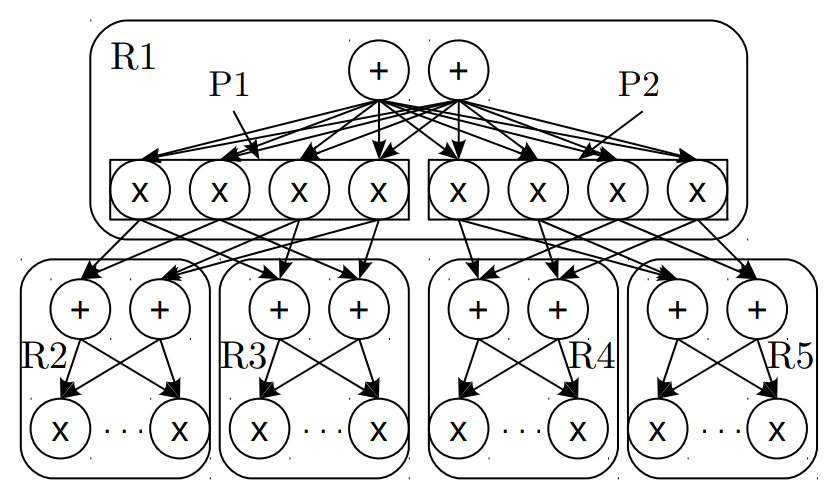
\includegraphics[scale=1.0]{imgs/trans_dv.png}
    \caption{}
  \end{subfigure}
  \captionsetup{justification=raggedright}
  \caption{A arquitetura de Dennis-Ventura gera um grafo de regiões (a) que representa um esboço da
    arquitetura real da rede soma-produto (b). Fonte:~\cite{clustering}}
\end{figure}

Após gerado o grafo de regiões, é feita uma transformação para uma rede soma-produto válida. Cada
nó região é transformado em um conjunto de $m$ nós somas. Se a região representa apenas um pixel,
então geram-se $g$ nós gaussianas, onde cada $q$-ésima gaussiana é o $q$-quantil do pixel. Para um
nó partição P, sejam $R_1$ e $R_2$ as duas subregiões filhas de $P$, e sejam $|R_1|$ e $|R_2|$ o
número de nós em cada filho do nó partição. São então criados $|R_1| |R_2|$ nós produtos, onde cada
aresta de $P$ é uma combinação dois a dois dos nós $R_1^i$ e $R_2^j$. O resultado desta
transformação é a arquitetura de Dennis-Ventura. Após criada a arquitetura, aprende-se os pesos
através do método de otimização de gradiente descendente.

O artigo de Gens e Domingos~\cite{gens-domingos} não explicíta o algoritmo em si. Ao invés disso, é
dado um esquema de algoritmo que garante uma estrutura profunda. Este esquema é chamado de
\code{LearnSPN}, e segue a ideia de que nós produtos representam independência entre as variáveis
envolvidas, enquanto que nós somas representam relações de semelhança entre as instâncias do
conjunto de dado.

\begin{algorithm}[H]
  \caption*{\code{LearnSPN}: Algoritmo de Gens-Domingos}
  \begin{algorithmic}[1]
    \Require\, Conjuntos $I$ de instâncias e $X$ de variáveis
    \Ensure\,SPN representando a distribuição de probabilidade de $I$ sobre as variáveis $X$
    \If{$|X|=1$}
      \State\,\textbf{retorna} distribuição de probabilidade univariada de $I$
    \Else%
      \State\,Particione $X$ em $P_1,P_2,\ldots,P_m$ tal que todo $P_i$ é independente de $P_j$,
      $i\neq j$
      \If{$m>1$}
        \State\,$\pi\gets$\mcode{Produto$()$}
        \For{$i\gets 1,\ldots,m$}
          \State\,\mcode{$p_i\gets$LearnSPN$(I, P_i)$}
          \State\,\mcode{$\pi$.AdicionaFilho$(p_i)$}
        \EndFor%
        \State\,\textbf{retorna} $\pi$
      \Else%
        \State\,Faça \textit{clustering} em $I$ tal que $Q_1,Q_2,\ldots,Q_n$ são os clusters de $I$
        \State\,$\sigma\gets$\mcode{Soma$()$}
        \For{$i\gets 1,\ldots,n$}
          \State\,\mcode{$s_i\gets$LearnSPN$(Q_i, X)$}
          \State\,$w\gets |Q_i|/|I|$
          \State\,\mcode{$\sigma$.AdicionaFilho$(s_i, w)$} \Comment{$w$ é o peso da aresta
            $\sigma\to s_i$}
        \EndFor%
        \State\,\textbf{retorna} $\sigma$
      \EndIf%
    \EndIf%
  \end{algorithmic}
\end{algorithm}

Para o algoritmo Gens-Domingos, separa-se o conjunto de dados $D$ em dois conjuntos $I$ e $X$ de
instâncias (por exemplo, imagens) e variáveis (ou seja, o escopo). O algoritmo é recursivo e pode
ser dividido em três partes: folha, produto e soma.

Para definir uma folha, apenas verifica-se se o conjunto de dados tem apenas uma variável como
escopo. Neste caso, retorna-se a distribuição de probabilidade univariada de $I$. Foram
implementadas duas versões desta parte. A primeira retorna como folha uma distribuição multinomial
com as frequências dos valores presentes em $I$. A segunda retorna uma distribuição gaussiana com
média e variância calculadas a partir de $I$.

Em seguida o algoritmo tenta construir um nó produto. Tomando-se $I$ e $X$, tenta-se particionar
$X$ em $P_1,P_2,\ldots,P_m$ partições, onde toda variável $Y\in P_i$ e $Z\in P_j$ obedece $Y\indep
X$ se e somente se $i\neq j$, onde $\indep$ representa independência. Foram implementados os testes
de $\chi^2$ e $G$-test para estatisticamente determinar se duas variáveis são independentes. No
entanto, testar cada variável par-a-par é intratável. Para resolver este problema, foi gerado um
grafo de independência, onde um vértice representa uma variável e uma aresta indica dependência
entre duas variáveis. Achar as partições de $X$ equivale a achar todas as componentes conexas do
grafo. Melhor do que isso, é fácil ver que é suficiente achar a árvore geradora mínima do grafo de
independência. Para isso, foi implementado o algoritmo de Kruskal para árvores geradoras mínimas.
As partições $P_1,\ldots,P_m$ equivalem às componentes conexas do grafo. Se $m>1$, então foram
encontradas relações de independência suficientes para construir um nó produto. Este nó produto tem
como filhos as chamadas recursivas de \code{LearnSPN} onde os escopos foram reduzidos às variáveis
de sua respectiva partição.

Caso $m=1$, então o grafo é conexo. Neste caso, gera-se uma soma. Faz-se o clustering de $I$ em
$Q_1,Q_2,\ldots,Q_n$ clusters. Foram implementadas versões que usam $k$-means, $k$-mode e
$k$-median para clusterização com número de clusters fixos. O algoritmo DBSCAN também foi
implementado. Este método de clustering baseado em densidade acha o número de clusters
automaticamente. Assim que os $Q_i$ clusters foram determinados, retorna-se um nó soma cujos filhos
são as chamadas recursivas com conjunto de instância restritas aos $Q_i$. Adicionalmente, o peso
das arestas do nó soma são as proporções dos tamanhos dos clusters.

Os testes de desempenho dos três algoritmos cobriram cinco conjuntos de dados.

\begin{enumerate}[label=\,(\alph*)]
  \item Caltech-101~\cite{caltech101}
  \item Olivetti Faces Dataset~\cite{olivetti}
  \item Digits~\cite{digits}
  \item DigitsX~\cite{digitsx}
  \item MNIST~\cite{mnist}
\end{enumerate}

O conjunto de dados Caltech-101 original\footnote{Disponível em
  \url{http://www.vision.caltech.edu/Image_Datasets/Caltech101/}.} contém imagens de 101 categorias
de objetos. As imagens têm diferentes dimensões e resoluções. Para os testes de desempenho do
projeto, as imagens foram padronizadas e redimensionadas para imagens em escala de cinza com
dimensões $150\times 65$ e quantizadas para uma resolução de 4-bits.  Adicionalmente, foram
escolhidas apenas as categorias moto, carro e rosto para classificação, as mesmas utilizadas para
os testes do artigo original~\cite{poon-domingos}.

\begin{figure}[h]
  \centering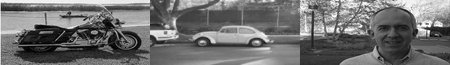
\includegraphics[scale=1.0]{imgs/caltech_sample.png}
  \caption{Uma amostra do conjunto de dados Caltech-101.}
\end{figure}

As imagens do Olivetti Faces Dataset\footnote{Disponível em
  \url{http://www.cl.cam.ac.uk/research/dtg/attarchive/facedatabase.html}} também foram
redimensionadas para imagens de tamanho $46\times 56$ com resolução 3-bits em escala de cinza. Este
conjunto de dados contém 10 fotos de rostos com ângulos e expressões diferentes de 40 pessoas
diferentes.

\begin{figure}[h]
  \centering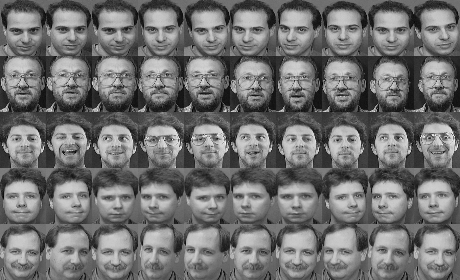
\includegraphics[scale=0.5]{imgs/olivetti_sample.png}
  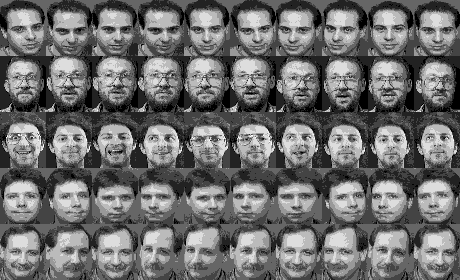
\includegraphics[scale=0.5]{imgs/olivetti-8_sample.png}
  \captionsetup{justification=raggedright}
  \caption{Uma amostra do conjunto de dados Olivetti. A imagem do lado esquerdo é uma amostra antes
    da redução de resolução. A imagem do lado direito mostra as imagens com resolução de 3-bits.}
\end{figure}

O par de conjuntos de dados
Digits\footnote{Disponível em \url{https://github.com/RenatoGeh/datasets/tree/master/digits}.} e
DigitsX\footnote{Disponível em \url{https://github.com/RenatoGeh/datasets/tree/master/digits_x}.}
contém imagens de dígitos de zero a nove. Apenas um tipo de caligrafia foi usado, e portanto as
imagens são semelhantes e têm baixa variância entre imagens de mesmo rótulo. Digits contém apenas
imagens binárias (preto ou branco), onde 1 indica cor branca e 0 indica cor preta. O conjunto
DigitsX é uma variação de Digits, onde cada imagem presente no conjunto original é transformada
numa imagem de 8-bits. Além disso, é aplicado um filtro de embaçamento gaussiano (gaussian blur)
para gerar maior variância e complexidade ao conjunto. São 70 imagens para cada dígito, dando um
total de 700 imagens para cada conjunto. Todas imagens de Digits e DigitsX têm dimensões $20\times
30$.

\begin{figure}[h]
  \centering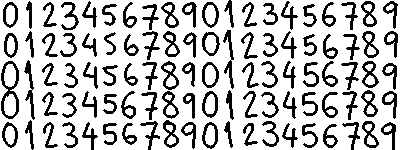
\includegraphics[scale=1.5]{imgs/digits_sample.png}
  \captionsetup{justification=raggedright}
  \caption{Amostras de cada dígito dos conjuntos Digits e DigitsX. A amostra do topo pertence ao
    conjunto Digits, onde cada pixel tem valor binário preto ou branco. A de baixo é a
    transformação das mesmas imagens de cima para o formato DigitsX.}
\end{figure}

MNIST é um conjunto de dados frequentemente usado para testar o desempenho de classificadores.
Assim como Digits, MNIST é um conjunto de dígitos de zero a nove escritos a mão. O conjunto
original contém 60000 imagens de treino e 10000 de teste, com aproximadamente 250 tipos de
caligrafia no conjunto de treino e 250 no de treino. Cada imagem tem dimensão $28\times 28$ e tem
valores binários. Foram escolhidas 2000 imagens de treino e 2000 de teste aleatoriamente para os
testes.

\begin{figure}[h]
  \centering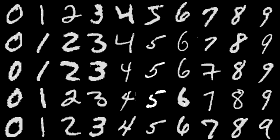
\includegraphics[scale=1.0]{imgs/mnist_sample.png}
  \captionsetup{justification=raggedright}
  \caption{Amostra de dígitos do conjunto MNIST\@. Ao contrário de Digits, os dígitos são escritos
    com valores representando branco, enquanto que o fundo é colorido com preto.}
\end{figure}

Foram feitos testes de classificação e compleição em todos os conjuntos de dados. O algoritmo de
Gens-Domingos admite tarefas de classificação e compleição sem alterar sua arquitetura, já que sua
estrutura independe do domínio das variáveis. Para os algoritmos de Poon-Domingos e Dennis-Ventura,
as redes geradas pelos algoritmos descritos nos artigos representam uma imagem, e adicionar
informação externa, como uma variável representando rótulos de classificação, requer modificar a
estrutura da rede. Para a tarefa de classificação nestes dois métodos de aprendizado, foi gerada
uma estrutura onde cada classe contém uma sub-SPN treinada a partir das instâncias do rótulo
correspondente.  Variáveis indicadoras da variável de classificação ``ligam'' e ``desligam'' as
sub-SPNs conforme a valoração da classificação.

\begin{figure}[h]
  \centering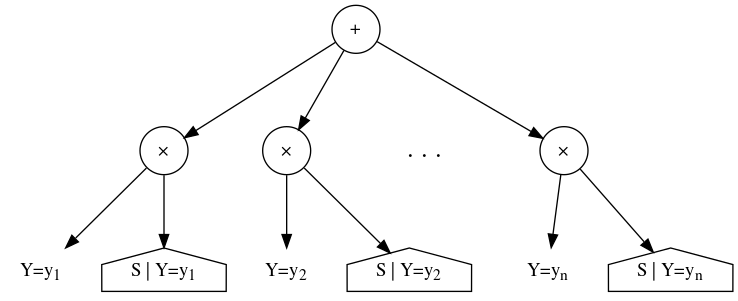
\includegraphics[scale=0.55]{graphs/classarch.png}
  \captionsetup{justification=raggedright}
  \caption{A arquitetura de classificação para os algoritmos de Poon-Domingos e Dennis-Ventura.
    Para cada valoração da variável de classificação $Y$, toma-se uma variável indicadora $Y_i$.
    O valor do nó produto ligado a $Y_i$ toma um valor 0 se $Y\neq y_i$, e $S|Y_i$ caso contrário.
    $S|Y=y_i$ representa uma SPN treinada com dados onde $Y$ teve valor $y_i$.}
\end{figure}

Para a tarefa de compleição de imagem nas arquiteturas de Poon-Domingos e Dennis-Ventura, foram
feitos testes tanto com as suas estruturas originais, onde as rotulações das classes não são
tomadas em consideração, quanto com as estruturas de classificação.

No artigo original de Hoifung Poon e Pedro Domingos~\cite{poon-domingos}, os testes feitos foram
executados em paralelo em um cluster de computadores onde cada máquina tinha 8 CPUs Intel Xeon
2.3GHz e 16GB de memória. Para os testes feitos neste projeto, foi usado apenas uma máquina com 4
CPUs Intel i7--4500U 1.8GHz. Enquanto que no artigo original durou-se 6 minutos para completar o
aprendizado do conjunto de dados Caltech-101 para todas as categorias, os testes feitos neste
projeto com o algoritmo de Poon-Domingos excederam mais de 24 horas para três categorias. Além
disso, enquanto que o artigo original usa 16 somas por região e 8 gaussianas por pixel, por
limitação de memória, tivemos de usar apenas 4 somas por região e 4 gaussianas por pixel. Devido a
esta discrepância em \textit{hardware} e tempo de execução, não foi possível apresentar resultados
para todos os testes usando a arquitetura de Poon-Domingos, e quando foi possível, os resultados
foram abaixo do esperado. O código do algoritmo de Poon-Domingos foi fortemente baseado no código
existente escrito em Java disponibilizado pelos autores do artigo. É possível que existam erros no
código, porém é também possível que os resultados ruins e longos tempos de execução se devam à
limitação de hardware e ao fato de ser necessário usar parâmetros bem menores. Será assinalado por
$\ast$ nas tabelas de teste quando algum algoritmo excedeu o tempo limite de 24 horas no teste.
Para os casos em que o algoritmo gastou mais de 16GB de memória, será usado o símbolo $\ast\ast$ na
tabela de testes.

Em questão de tempo de execução, o algoritmo de Gens-Domingos foi o mais rápido comparado aos
outros em conjuntos de dados com imagems pequenas. No entanto, sua complexidade aumenta
significantemente quando existe um número grande de categorias por variável ou quando a imagem é
grande. Isto ocorre pois o passo de determinar as partições de variáveis independentes ocupou 90\%
do tempo de execução do algoritmo, e os testes estatísticos de independência dependem fortemente do
número de categorias por variável e tamanho do escopo dos dados.  Por meio da quantização das
imagens (de 8-bit para 3 ou 4-bit), o tempo de execução diminuiu significantemente. Em comparação,
o algoritmo de Dennis-Ventura manteve-se mais constante em relação ao conjunto de dados, com
resultados melhores em tempo de execução ao de Gens-Domingos nos testes de Caltech-101 e Olivetti.
Como o método usa otimização de gradiente para determinar os pesos, o tempo de execução dependeu
mais fortemente do número de instâncias. O número de categorias para cada variável não teve impacto
no tempo de execução. O método de aprendizado de Poon-Domingos teve o maior tempo de execução em
todos os testes. Como cada iteração do algoritmo demora cerca de 15 minutos e todos conjuntos de
dados contém mais de 300 instâncias, não foi possível extrair resultados de todos os conjuntos para
o algoritmo de Poon-Domingos.

As tabelas de acurácia mostram a porcentagem de acertos que cada algoritmo apresentou no conjunto.
A linha ``Partição $p$'' indica a porcentagem $p$ do conjunto de dados usado para treino e $1-p$
para teste. Portanto, se $p=0.7$ no conjunto DigitsX, serão usadas 490 imagens para treino e os 210
restantes para teste. Cada partição tem número uniforme de imagens para cada rótulo de
classificação. Para o conjunto MNIST, como existem conjuntos de treino e teste separados, não houve
partição. Ao invés disso, foram feitas classificações in-sample, onde faz-se a união do conjunto de
treino e teste e em seguida toma-se aleatoriamente metade desta união como treino e o restante como
teste, e classificação out-sample, onde toma-se apenas o conjunto de treino para treino e o de
teste para teste. Todos os valores de acurácia são em porcentagem de acerto.

\begin{table}[H]
  \centering\textbf{DigitsX}\vspace{0.25cm}
  \begin{tabular}{l|cccccccccc}
    Partição $p$ & $0.1$ & $0.2$ & $0.3$ & $0.4$ & $0.5$ & $0.6$ & $0.7$ & $0.8$ & $0.9$\\
    \hline
    Poon-Domingos & $10.0$ & $10.0$ & $\ast$ & $\ast$ & $\ast$ & $\ast$ & $\ast$ & $\ast$ & $\ast$\\
    Dennis-Ventura & $92.85$ & $98.57$ & $99.18$ & $98.81$ & $99.42$ & $99.28$ & $98.57$ & $93.33$ & $88.75$\\
    Gens-Domingos & $91.27$ & $96.78$ & $96.93$ & $98.09$ & $97.14$ & $97.85$ & $97.61$ & $92.66$ & $86.25$\\
  \end{tabular}\\~\\
  \textbf{Caltech-101}\vspace{0.25cm}\\
  \begin{tabular}{l|cccccccccc}
    Partição $p$ & $0.1$ & $0.2$ & $0.3$ & $0.4$ & $0.5$ & $0.6$ & $0.7$ & $0.8$ & $0.9$\\
    \hline
    Poon-Domingos & $\ast\ast$ & $\ast\ast$ & $\ast\ast$ & $\ast\ast$ & $\ast\ast$ & $\ast\ast$ & $\ast\ast$ & $\ast\ast$ & $\ast\ast$\\
    Dennis-Ventura & $78.58$ & $78.49$ & $80.28$ & $79.88$ & $81.38$ & $81.35$ & $75.45$ & $74.78$ & $75.75$\\
    Gens-Domingos & $77.40$ & $85.00$ & $84.28$ & $86.11$ & $88.66$ & $90.00$ & $92.22$ & $90.00$ & $84.84$\\
  \end{tabular}\\~\\
  \textbf{Olivetti}\vspace{0.25cm}\\
  \begin{tabular}{l|cccccccccc}
    Partição $p$ & $0.1$ & $0.2$ & $0.3$ & $0.4$ & $0.5$ & $0.6$ & $0.7$ & $0.8$ & $0.9$\\
    \hline
    Poon-Domingos & $10.0$ & $\ast\ast$ & $\ast\ast$ & $\ast\ast$ & $\ast\ast$ & $\ast\ast$ & $\ast\ast$ & $\ast\ast$ & $\ast\ast$\\
    Dennis-Ventura & $83.78$ & $74.88$ & $89.85$ & $89.93$ & $96.22$ & $97.50$ & $92.89$ & $50.00$ & $60.93$\\
    Gens-Domingos & $2.50$ & $2.50$ & $93.92$ & $91.25$ & $95.50$ & $98.75$ & $81.93$ & $81.59$ & $100.0$\\
  \end{tabular}\\~\\
  \textbf{MNIST}\\(2000 treino / 2000 teste)\vspace{0.25cm}\\
  \begin{tabular}{l|ccc}
    Classificação & Poon-Domingos & Dennis-Ventura & Gens-Domingos \\
    \hline
    In-sample & $\ast$ & $77.85$ & $81.55$ \\
    Out-sample & $\ast$ & $69.90$ & $76.90$ \\
  \end{tabular}
\end{table}

No quesito acurácia na tarefa de classificação, o algoritmo de Gens-Domingos teve os melhores
resultados em média. Em seguida, Dennis-Ventura alcançou, em média, resultados comparáveis ao
primeiro algoritmo. Por último, o de Poon-Domingos apresentou os piores resultados. Observou-se que
Gens-Domingos tem melhores resultados quando existe um grande número de dados para treino. O
algoritmo de Dennis-Ventura conseguiu bons resultados com poucos dados. Conjectura-se que, como
Dennis-Ventura tem uma estrutura voltada para domínios parecidos com o de imagens, é esperado que
tenha bons resultados com poucos dados. Enquanto isso, o algoritmo de Gens-Domingos tem aplicações
mais gerais, além de ser um método de aprendizado estrutural, o que requer mais informação para
gerar uma estrutura mais informativa e que capture melhor as interações entre variáveis.

Para os testes de compleição de imagem, dois parâmetros foram definidos. O parâmetro de
conhecimento de classe (CC) indica se o teste de compleição admite que a SPN tenha conhecimento da
classe a ser completada. Por exemplo, no conjunto Olivetti existem 40 classes, onde cada classe
corresponde a uma pessoa. Cada classe contém 10 instâncias de rostos. Com conhecimento de classe, o
teste de compleição para uma instância $I$ de uma classe $c$ no conjunto $D$ será avaliado com uma
SPN treinada com o conjunto de dados $D\setminus\{I\}$, ou seja, a SPN terá conhecimento do rosto
da pessoa cuja imagem será completada. Sem conhecimento a priori de classe o teste é feito com uma
SPN treinada com o conjunto $D\setminus\{I\}, \forall I$ tal que $I[C]=c$, ou seja, com o conjunto
de todas as imagens cujos rostos não pertençam a pessoa $c$. O segundo parâmetro, chamado de
conhecimento de rótulo (CR) indica se, durante a compleição de uma imagem $I$, foi dada como parte
da evidência o rótulo da imagem a ser completada. O parâmetro CC tenta avaliar o quão bem a SPN
generaliza os dados quando se é dada informação nunca vista pelo modelo, enquanto que o parâmetro
CR avalia se o teste depende da classificação da classe para gerar uma boa compleição.

As compleições foram geradas tomando como evidência metade da imagem e em seguida computando a
hipótese mais provável (MPE, de \textit{Most Probable Explanation}) que o modelo assume. A MPE de
uma evidência é computada de forma aproximada usando a rede máximo-produto do modelo. O resultado
do MPE é um conjunto de valorações das variáveis de todos os pixels da imagem, onde a metade usada
como evidência permanece inalterada e a outra metade representa a compleição. Nos testes feitos
neste projeto, coloriu-se em escala de verde a compleição feita pela SPN, enquanto que a metade
tomada como evidência foi mantida em escala de cinza. Uma linha vermelha de um pixel de largura foi
traçada para separar as partições.

\begin{figure}[h]
  \centering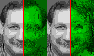
\includegraphics[scale=5.0]{cmpl/dennis/face_0.png}
  \caption{Compleição de uma imagem do conjunto de dados Olivetti usando o algoritmo de
    Dennis-Ventura. A compleição da esquerda usa compleição de classe (CC), enquanto que o da
    direita não.\label{fig:cmpl_0}}
\end{figure}

Analisando as imagens, foi possível perceber que o parâmetro CR não teve impacto nas compleições,
já que na maior parte das vezes o algoritmo já classificava o rótulo correto. O parâmetro CC teve
maior impacto. Como a SPN não tem conhecimento de características que apenas uma classe possue, o
modelo tentou utilizar características de outras classes, gerando faces desproporcionais, como na
\autoref{fig:cmpl_0}.

As tarefas de compleição mostraram que a SPN identificou características comuns entre várias
classes. Por exemplo, no conjunto Olivetti, a SPN conseguiu reconstruir partes do corpo como nariz,
olhos e bigode de forma razoável. Em alguns casos, a rede teve dificuldade com a presença ou
ausência de óculos e barba.

\begin{figure}[h]
  \centering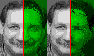
\includegraphics[scale=21.0]{cmpl/gens/face_0.png}
  \caption{Compleição da mesma face da~\autoref{fig:cmpl_0} usando o algoritmo Gens-Domingos. A
    imagem da esquerda possue conhecimento de classe e a da esquerda não.}
\end{figure}

O algoritmo de Gens-Domingos apresentou melhores resultados na tarefa de compleição. Algumas
imagens completadas pelo algoritmo Dennis-Ventura não apresentaram características fortes (como
nariz, boca ou olhos) mas tinham o formato certo de rosto e cabelo. Certas compleções parecem ter
parte das faces faltando, enquanto que outras possuem mais de dois olhos. A~\autoref{fig:cmpl_1}
contém algumas das piores compleições.

A boa performance do algoritmo Gens-Domingos mostra que talvez a estrutura da rede seja mais
importante do que adequar os pesos do modelo aos dados. Além disso, o algoritmo de Gens-Domingos
apresentou resultados bem melhores na compleição comparado ao de Dennis-Ventura, o que mostra que o
primeiro algoritmo parece ser melhor em tarefas generativas. Enquanto isso, em tarefas
discriminativas como classificação, os dois algoritmos tiveram resultados semelhantes.

\begin{figure}[H]
  \centering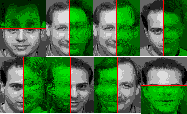
\includegraphics[scale=2.5]{cmpl/notfine/notfine.png}
  \caption{Compleições com características faciais faltando ou fora do padrão. Nestes casos a rede
    não conseguiu identificar olhos, nariz orelhas ou bocas de forma ideal.\label{fig:cmpl_1}}
\end{figure}

Por questão de tempo e limitação de número de páginas do relatório, foram apenas mostradas
compleições do conjunto de dados Olivetti. No entanto, é possível replicar os testes de
classificação e compleição de imagens usando o código presente em
\url{https://github.com/RenatoGeh/benchmarks}. Outras compleições do conjunto Olivetti também podem
ser vistas em \url{https://github.com/RenatoGeh/gospn/tree/dev/results/olivetti_3bit}.

\section{Conclusão}

Redes soma-produto são modelos probabilísticos baseados em grafos que representam distribuições de
probabilidade tratáveis. Neste projeto foram feitas comparações no domínio de classificação e
compleição de imagem entre três métodos de aprendizado estado-da-arte de redes soma-produto. Além
disso, planejou-se implementar e disponibilizar uma biblioteca livre e gratuita para inferência e
aprendizado de redes soma-produto.

Foram implementados três algoritmos de aprendizado. No entanto, apenas dois geraram bons
resultados. Devido à limitações de tempo e memória, e possivelmente erros no código, o terceiro
algoritmo não rodou de forma ótima. Em tarefas de classificação, os algoritmos que apresentaram
resultados mostraram boa acurácia em conjuntos de dados reais e artificiais, como identificação de
dígitos manuscritos, classificação de faces e de objetos, mesmo quando os conjuntos de dados
continham poucos dados de treino. Na tarefa de compleição, o modelo conseguiu identificar
características importantes das imagens, e conseguiu as replicar de forma razoável, mesmo quando as
imagens continham informações nunca antes vistas.

Todo o código é aberto e foi implementado e disponibilizado de forma livre e gratuita em
\url{https://github.com/RenatoGeh/gospn} com licensa BSD-3-Clause. A biblioteca inclue
documentação, funções para computar inferência, manipular conjuntos de dados e analisar acurácia em
classificação e compleição de imagens, além de três algoritmos de aprendizado de redes soma-produto
implementados com parâmetros ajustáveis, como diferentes variações para clusterização e testes de
independência de variável.

\printbibliography[]

\end{document}
